\documentclass[12pt]{article}%
\usepackage{amsfonts}
\usepackage{fancyhdr}
\usepackage{comment}
\usepackage[a4paper, top=2.5cm, bottom=2.5cm, left=2.2cm, right=2.2cm]%
{geometry}
\usepackage{pdfpages}
\usepackage{times}
\usepackage{amsmath}
\usepackage{changepage}
\usepackage{amssymb}
\usepackage{graphicx}%
\setcounter{MaxMatrixCols}{30}
\newtheorem{theorem}{Theorem}
\newtheorem{acknowledgement}[theorem]{Acknowledgement}
\newtheorem{algorithm}[theorem]{Algorithm}
\newtheorem{axiom}{Axiom}
\newtheorem{case}[theorem]{Case}
\newtheorem{claim}[theorem]{Claim}
\newtheorem{conclusion}[theorem]{Conclusion}
\newtheorem{condition}[theorem]{Condition}
\newtheorem{conjecture}[theorem]{Conjecture}
\newtheorem{corollary}[theorem]{Corollary}
\newtheorem{criterion}[theorem]{Criterion}
\newtheorem{definition}[theorem]{Definition}
\newtheorem{example}[theorem]{Example}
\newtheorem{exercise}[theorem]{Exercise}
\newtheorem{lemma}[theorem]{Lemma}
\newtheorem{notation}[theorem]{Notation}
\newtheorem{problem}[theorem]{Problem}
\newtheorem{proposition}[theorem]{Proposition}
\newtheorem{remark}[theorem]{Remark}
\newtheorem{solution}[theorem]{Solution}
\newtheorem{summary}[theorem]{Summary}
\newenvironment{proof}[1][Proof]{\textbf{#1.} }{\ \rule{0.5em}{0.5em}}

\newcommand{\Q}{\mathbb{Q}}
\newcommand{\R}{\mathbb{R}}
\newcommand{\C}{\mathbb{C}}
\newcommand{\Z}{\mathbb{Z}}

\begin{document}

    \title{CS280 Spring 2023 Assignment 3 \\ Part A}
    \author{RNN, LSTM and GRU}
    \maketitle

    \paragraph{Name:} Bingnan Li

    \paragraph{Student ID:} 2020533092

    \newpage


    \subsubsection*{1. Parity-check network (16 points)}
    Note that the initial parity bit is 1, what's the relation between each input and the previous parity bit? Determine the relation between the parity and inputs and complete the parity bits($p_1,p_2,p_3,p_4$) and design and draw a RNN to predict parity.

    \begin{align*}f
        \textit{Parity bits}&:\quad\quad0\quad0\quad0\quad1\quad0\quad1\quad p_1\quad p_2\quad p_3 \quad p_4 \quad\rightarrow \\
        \textit{Input}&:\quad\quad0\quad1\quad1\quad0\quad0\quad0\quad1\qquad1\quad0\qquad0
    \end{align*}
    \begin{solution}
        The relation between the parity and inputs is that the parity bit $p_i$ is 1 if the number of 0s from $x_0$ to $x_i$ is even and 0 if the number of 0s from $x_0$ to $x_i$ is odd.
        With the formula above, we can get the parity bits as follows:
        $p_1 = 1,\ p_2 = 1,\ p_3 = 0,\ p_4 = 1$.
        The corresponding RNN is shown in Figure~\ref{fig:RNN}.
        \begin{figure}[htbp]
            \centering
            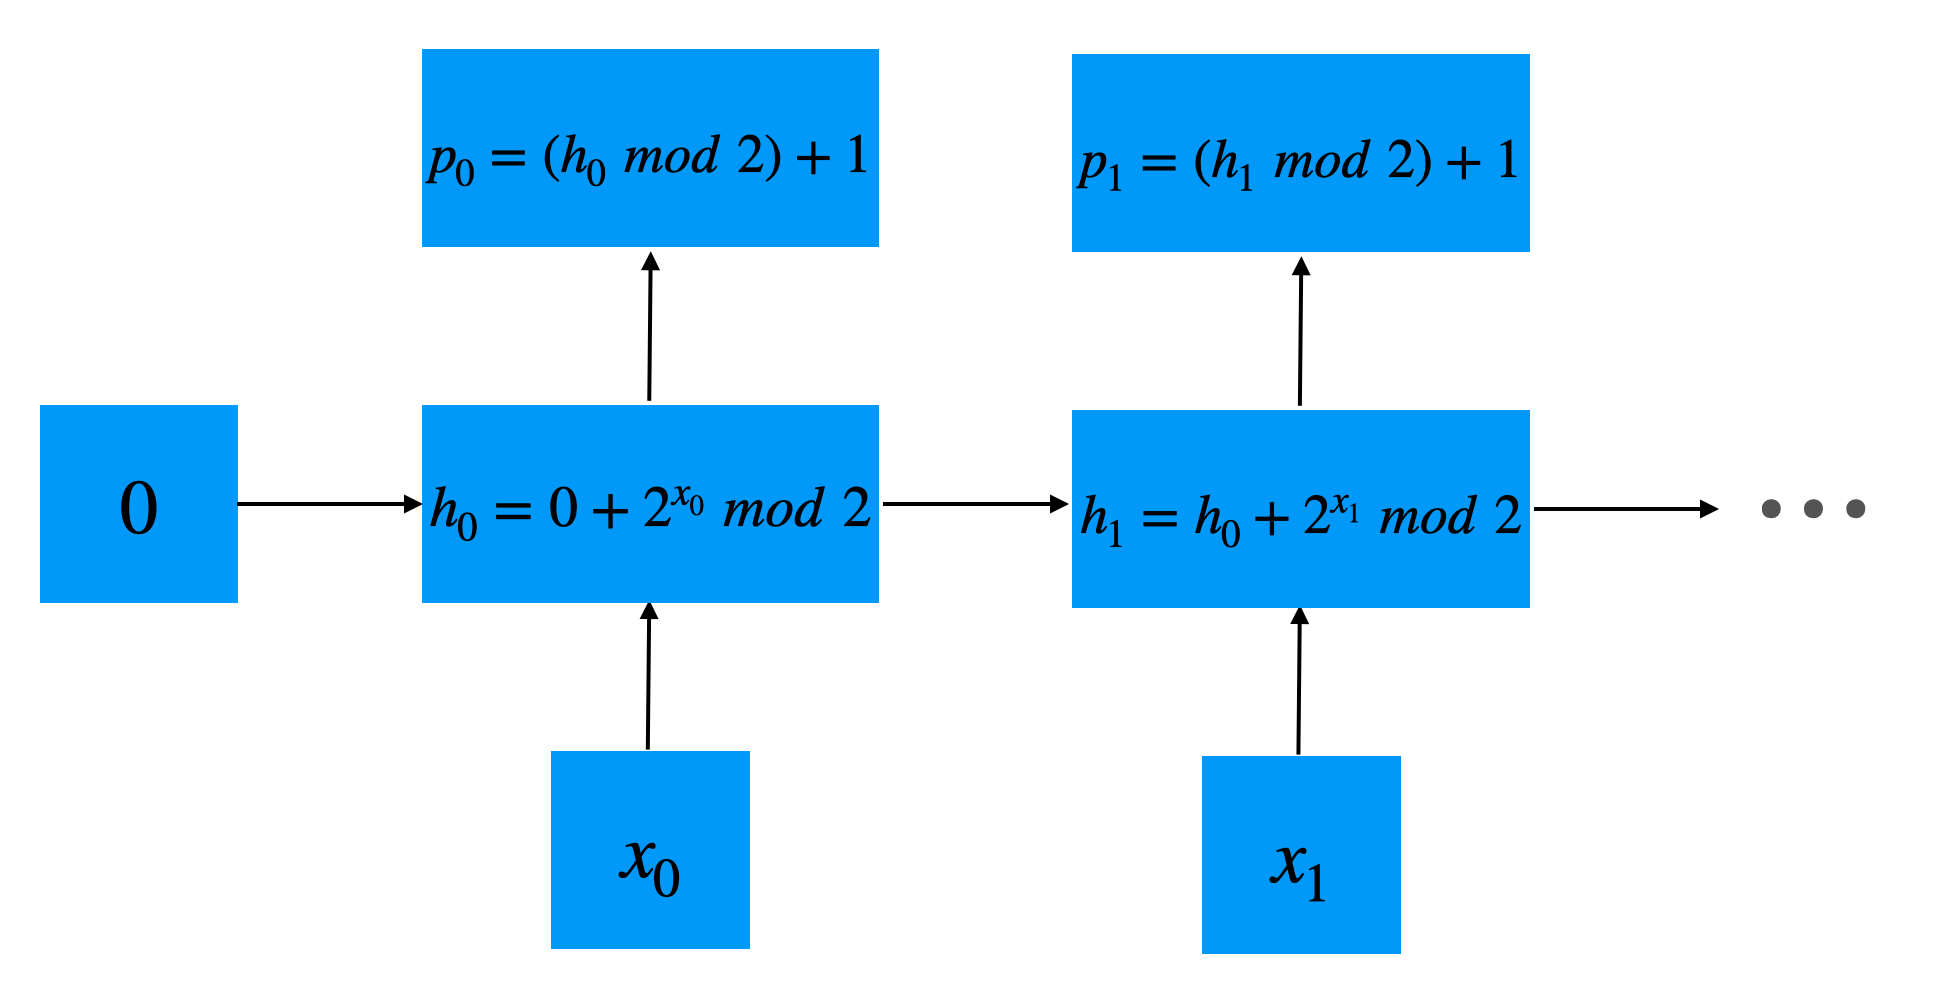
\includegraphics[width=0.8\textwidth]{images/partA_p1}
            \caption{RNN}
            \label{fig:RNN}
        \end{figure}
    \end{solution}


    \newpage


    \subsubsection*{2. GRU (17 points)}

    1. Please describe the forward propagation process of LSTM, and analyze the reasons for the disappearance of gradient.\\
    2. Please describe the differences between LSTM and GRU.\\
    3. Please provide examples of scenarios where GRU and LSTM are used respectively. Explain your reason.

    \begin{solution}
        \begin{itemize}
            \item [  ]
            \item [1.] The LSTM takes the current input $x_t$, previous cell state $C_{t-1}$ and hidden state $h_{t-1}$ as inputs.
            The forward process consists three parts: forget gate, input gate and output gate.
            \par {\bf Forget gate:} This gate takes in $x_t$ and $h_{t-1}$ and output $f_t$ which determines how much information is removed from $C_{t-1}$.
            The corresponding formula is \[f_t = \delta(W_f[h_{t-1},x_t])+b_f\] where $\delta$ is the sigmoid function, $W_f,b_f$ are the weight matrix and the bias term.
            \par {\bf Input gate:} This gate takes in $x_t$ and $h_{t-1}$ and output new cell information $\widetilde{C}_{t}$ and $i_t$ which determines how much information is added into cell state.
            The corresponding formula is \[i_t = \delta(W_i[h_{t-1},x_t]+b_i)\qquad \widetilde{C}_t=\tanh(W_C[h_{t-1},x_t]+b_C)\]
            \par {\bf Cell state update:} This process utilizes $f_t,C_{t-1},i_t,\widetilde{C}_t$ to output the new cell state $C_t$ with formula:
            \[C_t = f_t\cdot C_{t-1} + i_t\cdot \widetilde{C}_t\]
            \par {\bf Output gate:} This gate takes in $x_t$, $h_{t-1}$ and $C_t$ and output the new hidden state $h_{t}$ and $o_t$ which determines how much information is used to generate $h_t$.
            The corresponding formula is \[o_t = \delta(W_o[h_{t-1},x_t]+b_o))\qquad h_t=o_t\cdot \tanh(C_t)\]
            \par {\bf Why gradient vanish?} Consider the gradient of $C_t$, by chain rule, we have \[\bar{C}_t=\bar{C}_{t+1}\frac{\partial f_{t+1}C_t+i_{t+1}\widetilde{C}_{t+1}}{\partial C_t}=\bar{C}_{t+1}f_{t+1}\]
            Thus, \[\bar{C}_1=\bar{C}_T\prod_{i=2}^T f_i\]
            When one of the $f_i$ is $0$ or all the $f_i$s are very small, then the gradient will goes to 0.
            \item [2.] GRU is a simplified variant of LSTM with three main modifications:
            \begin{enumerate}
                \item GRU combines the forget and input gate into an update gate.
                \item GRU combines the cell state and the hidden state.
                \item GRU resets the previous hidden state before using it to extract the new information from the current input.
            \end{enumerate}
            \item [3.] GRU is used when we require the performance and the input sequence is relatively short while LSTM is used when the input sequence is much longer.
            This is because GRU is simpler and has much faster inference time.
            Moreover, since GRU combines the cell state with hidden state, the long memory capability will be relatively weaker than LSTM\@.
        \end{itemize}
    \end{solution}

    \newpage
    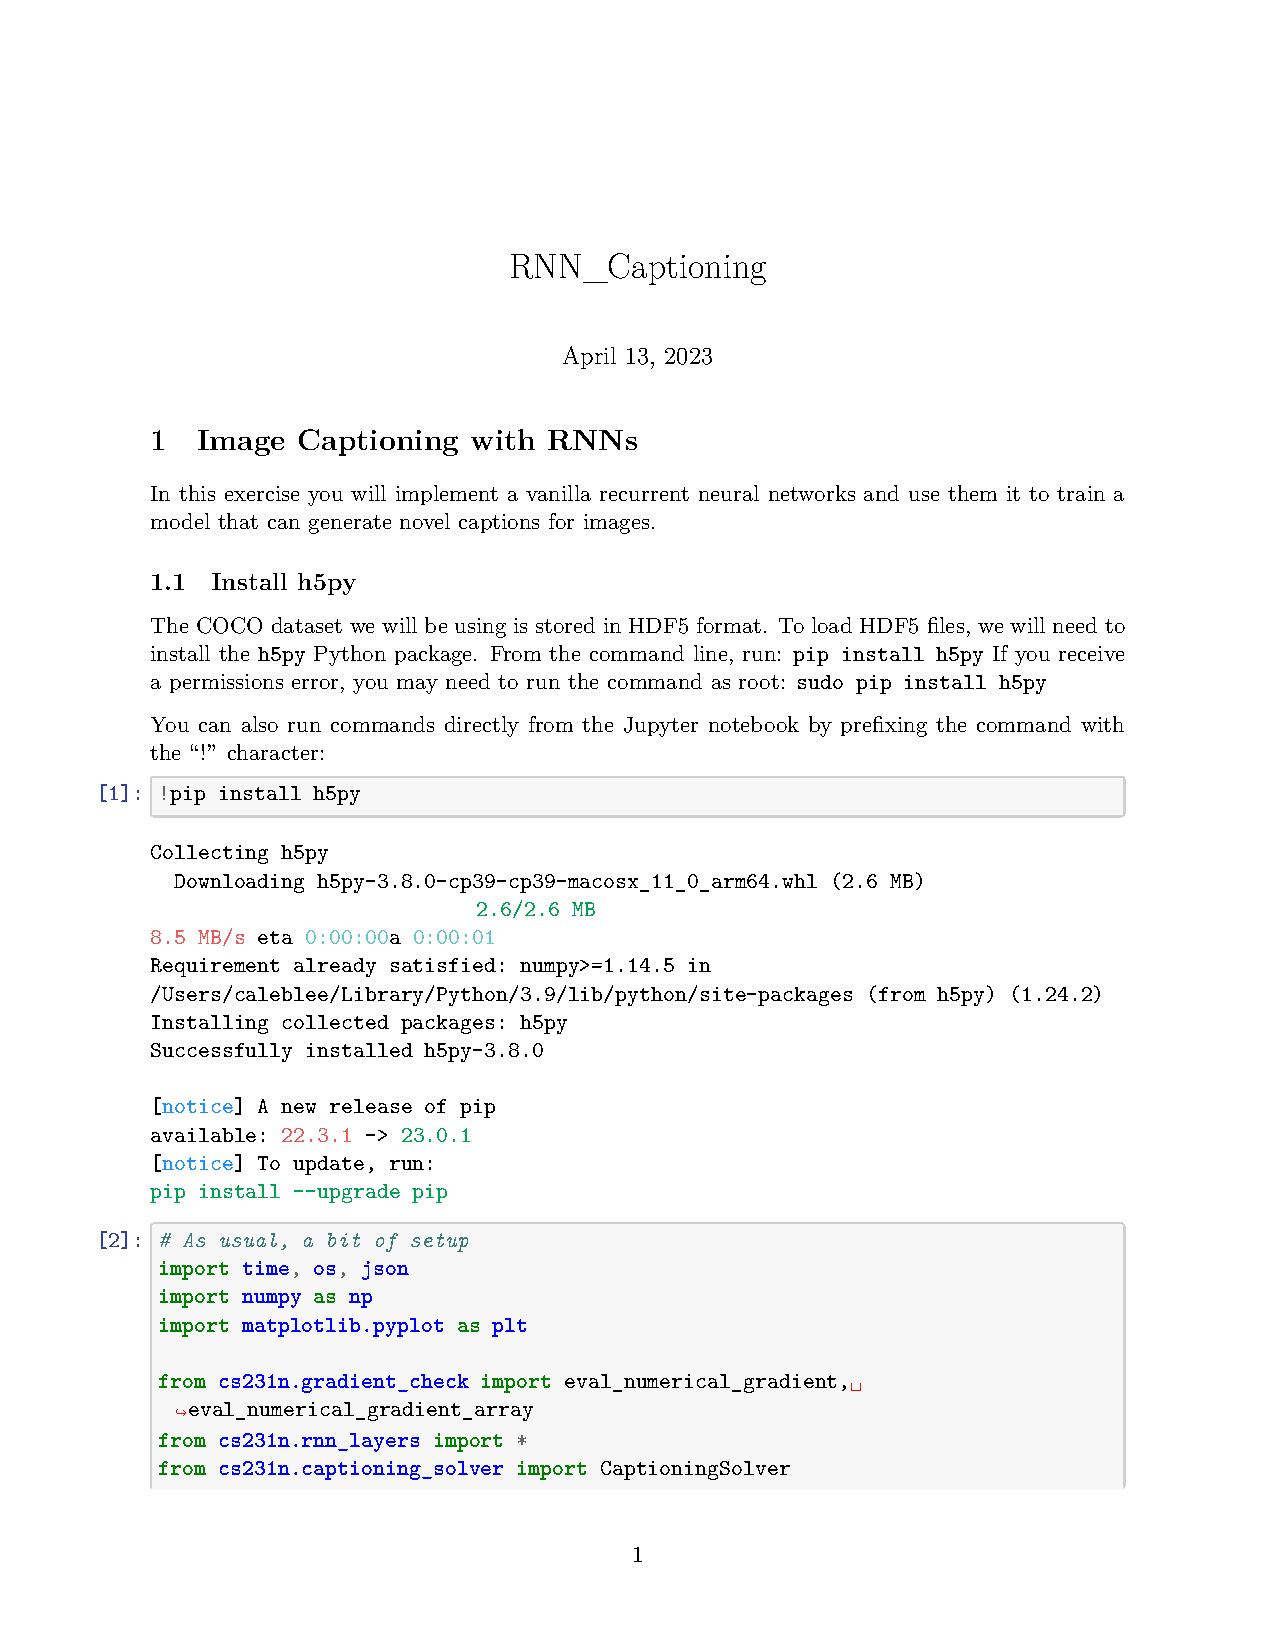
\includepdf[pages=1-]{RNN_Captioning.pdf}
    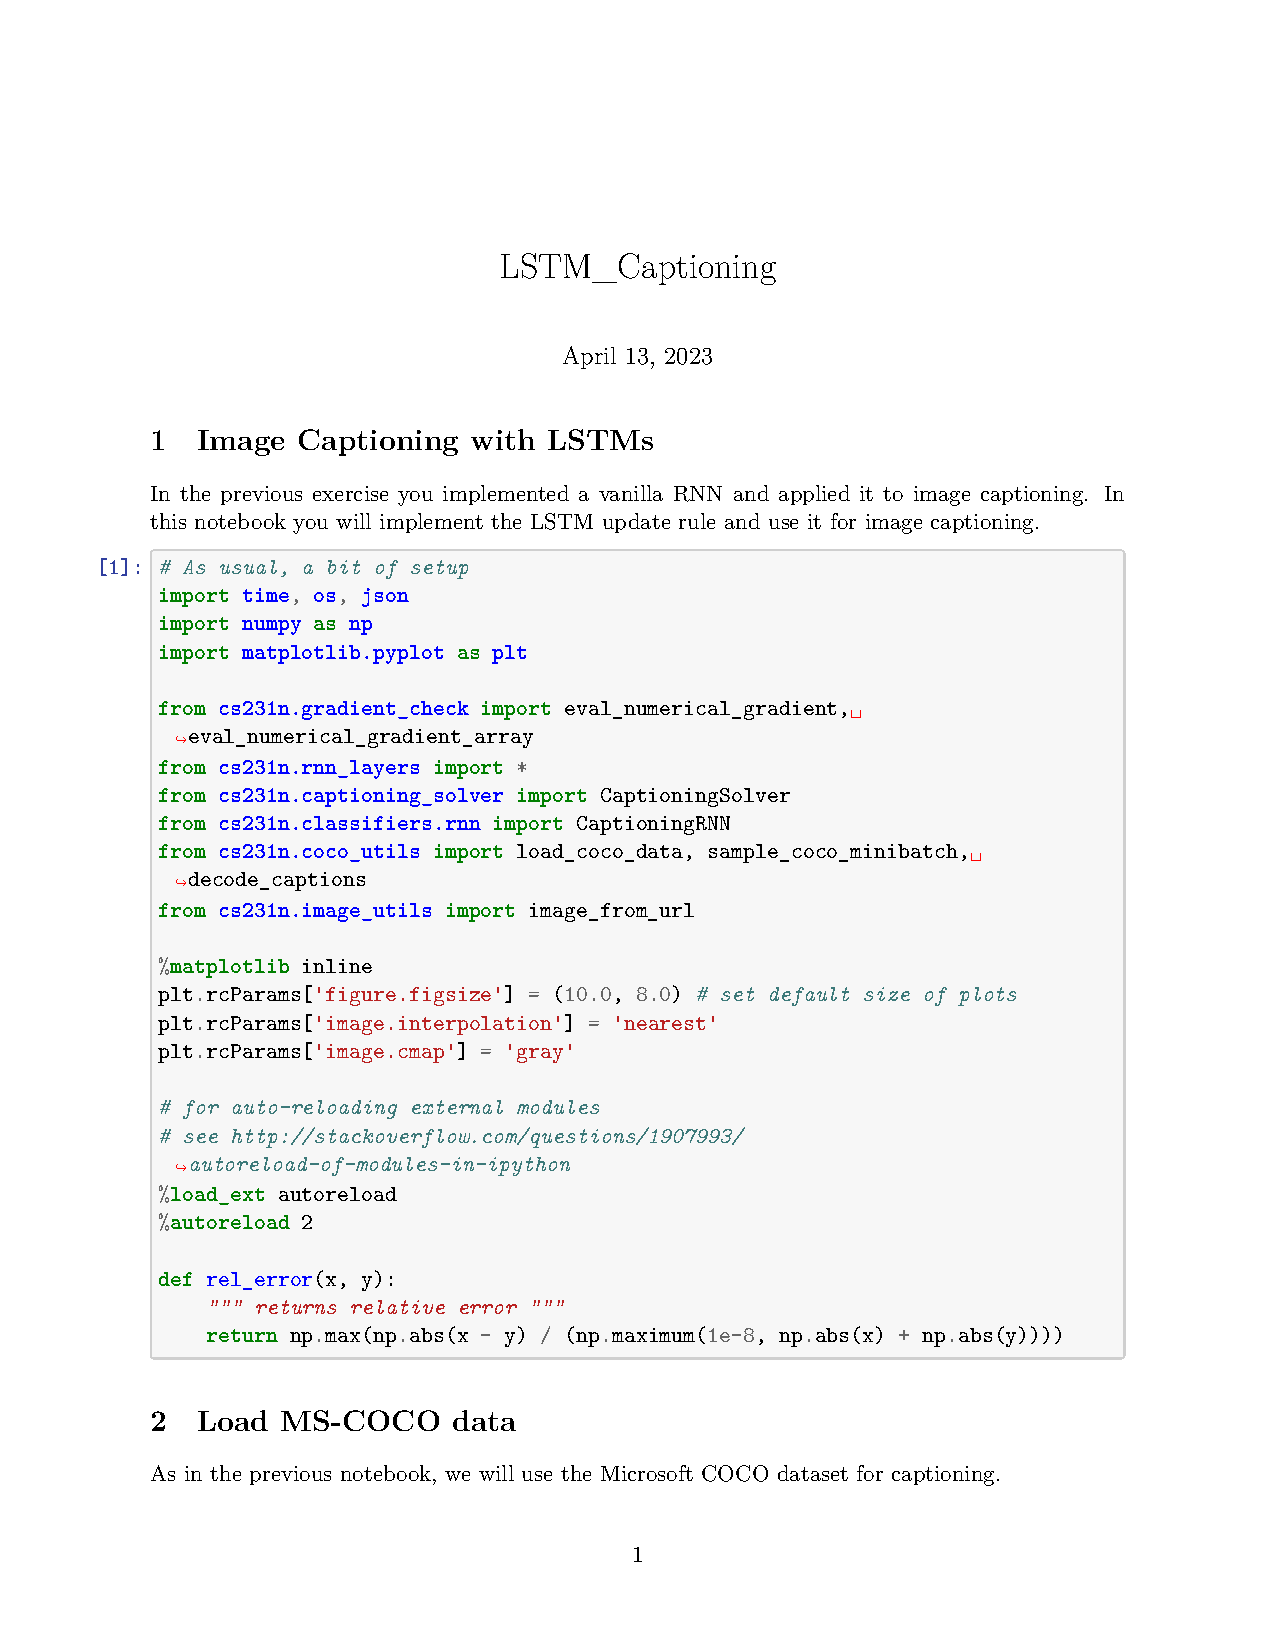
\includepdf[pages=1-]{LSTM_Captioning.pdf}
    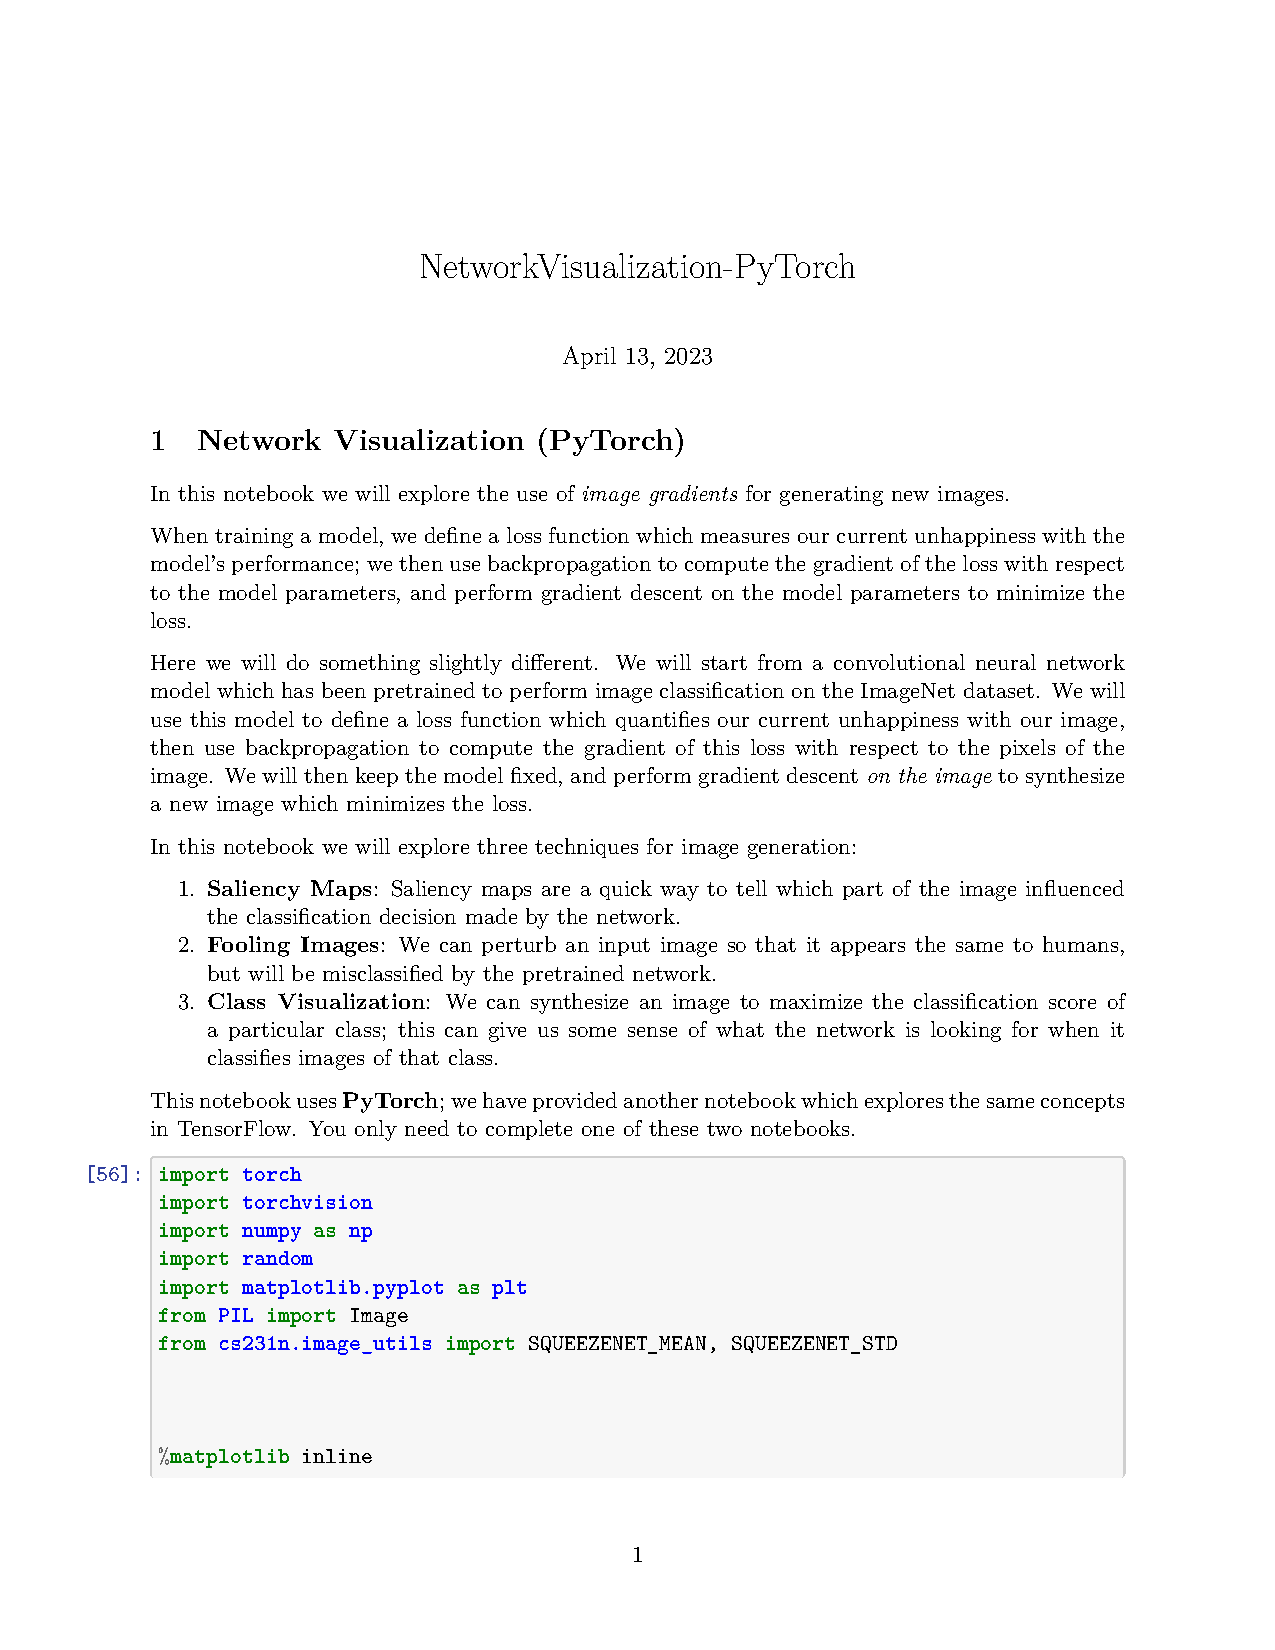
\includepdf[pages=1-]{NetworkVisualization-PyTorch.pdf}

\end{document}